\linespread{0.87}

%--------Cabeçalho do documento
\noindent\begin{minipage}[c][1.5cm][c]{3.5cm}
%\includegraphics[height=1.5cm]{./figuras/logoEvangelica.eps}

\includegraphics[width=1.5 \textwidth]{./outros/fig/IFGAnapolisHor2.png}
\end{minipage}\quad\quad\quad\qquad
\begin{minipage}{12cm}%10cm
\scriptsize\textbf{\ministerio}\\%\sc
\textbf{\secretaria}\\
\textbf{\instituto}\\
\textbf{\reitoria}\\
\end{minipage}
\vspace{1cm}
%---------------------------------------------------------------------------------------


\begin{center}
	\textbf{ATA N\textsuperscript{o} 20/2022.1}\\
	\footnotesize{\MakeUppercase{\textbf{Ata da sess\~ao p\'ublica de apresenta\c{c}\~ao do trabalho de conclus\~ao de curso 2}}}
\end{center}
\vspace{1.0cm}
\noindent Aos~0\diaata~dias do m\^es de~\mesata~do ano de dois mil e vinte dois, \'as~\hinicial~horas, por meio de webconfer\^encia utilizando Google Meet, foi realizada a sess\~ao p\'ublica de apresenta\c{c}\~ao do Trabalho de Conclus\~ao 2 da Graduando~\textbf{\alunonome~\alunosobre}~(matr\'icula~\matricula) do curso de~\curso. A banca foi composta pelos seguintes membros:~\orientadora,~\membroum,~\membrodois, sob a presid\^encia da primeira. O trabalho de conclus\~ao de curso tem como t\'itulo ``\textbf{\titulo}'', da \'area de Geotecnia, sob orienta\c{c}\~ao da Prof\textsuperscript{a}~\orientadora. Ap\'os a apresenta\c{c}\~ao do Trabalho de Conclus\~ao de Curso 2, tendo sido o autor arguido pela Banca Examinadora, a nota obtida foi~\notanumerico~(\notaextenso).
\\
\\
\noindent Encerra-se a presente sess\~ao \'as~\hfinal~horas~e~\mfinal~minutos. Eu Prof\textsuperscript{a}.~\orientadora, dato e assino a presente ata que segue assinada por todos os membros da Banca e pelo graduando.
\vspace{1.0cm}
\small{
\begin{center}
\begin{tabular}{c}
\multicolumn{1}{c}{\asseletronica} \\ 
\multicolumn{1}{c}{Prof\textsuperscript{a}~\orientadora} \\ 
\multicolumn{1}{c}{} \\ 
\asseletronica \\ 
\multicolumn{1}{c}{Prof\textsuperscript{a}~\membroum~} \\ 
\multicolumn{1}{c}{~} \\ 
\asseletronica\\
%
\includegraphics[width=0.30 \textwidth]{./outros/fig/AssDaniel.jpg} \\ %\hrulefill comando para linha
\multicolumn{1}{c}{Prof\textsuperscript{a}~\membrodois~} \\ 
\multicolumn{1}{c}{~} \\ 
\includegraphics[width=0.25 \textwidth]{./outros/fig/minhaAssinatura.png} \\
\multicolumn{1}{c}{\textbf{\alunonome~\alunosobre}} \\
\multicolumn{1}{c}{(Graduando)} \\
\multicolumn{1}{c}{~} \\ 
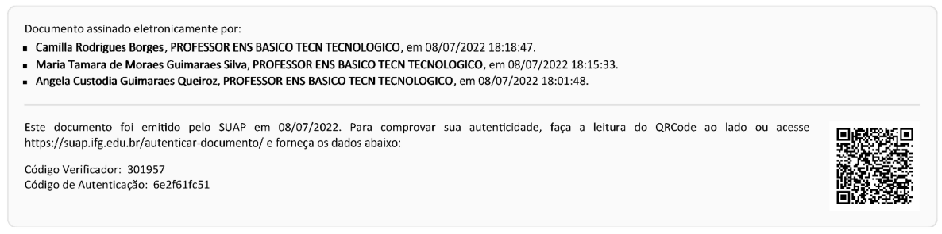
\includegraphics[width=0.97 \textwidth]{./outros/fig/QR_CODE_V2.pdf}
\\
\end{tabular}
\end{center}
}

\linespread{1.3}
\newpage


